%i am a comment!
\documentclass[11pt]{article}
\usepackage{fullpage}
\usepackage{graphicx}


\title{Latex Sample File}

\author{
James Parker\\jparker@cs.umn.edu
}
\date{\today}

\begin{document}

\maketitle

\section{Figures}
\label{sec:fig}

Please don't write on walls as seen in Figure~\ref{fig:tabl} in Section~\ref{sec:fig}.
   \begin{figure}[h] % "h" is where to place, h=here, t=top, b=bottom
      \centering
      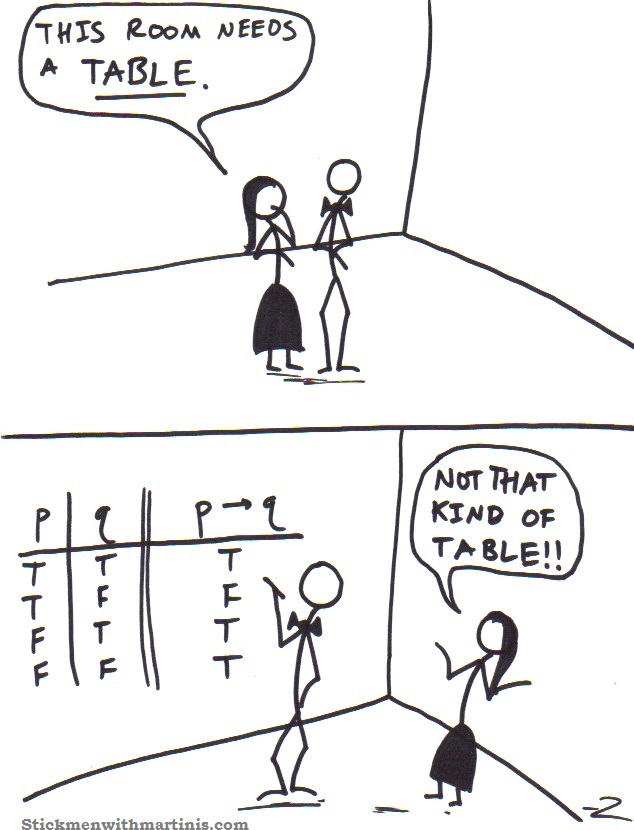
\includegraphics[height=80mm]{truth-table.jpg}
      \caption{I am a caption.}
      \label{fig:tabl}
   \end{figure}


% star does not give section with number
\section*{Tables}

Prisoner's Dillema: see Table \ref{tab:pd}.

\begin{table}
\centering
\caption{Prisoner's Dilemma}
\begin{tabular}{| l || c | c |} %sets the format of the table
\hline %horizontal line
 & Confess & Lie \\ % the "&" separates parts based on the format above
   \hline \hline
Confess & (-8, -8) & (0, -10) \\ % the "\\" makes it go down a line (i.e. done with line)
\hline
Lie & (-10, 0) & (-1, -1) \\ 
\hline
   \end{tabular}
\label{tab:pd} 
\end{table}


\end{document}
